\documentclass[a4paper, 11pt]{article}
\usepackage[utf8]{inputenc}

\usepackage[breaklinks, colorlinks=true, citecolor=black, linkcolor=blue, urlcolor=blue, filecolor=blue]{hyperref}

\usepackage{comment}

\usepackage[center, labelfont=bf]{caption}
\captionsetup{justification=justified, singlelinecheck=false} % Justify left

\usepackage{amsmath} % Math equation

% For table
\usepackage{multirow}
\usepackage[table, xcdraw]{xcolor}

% Page definitions
\setlength{\topmargin}{1.5cm}
\setlength{\headheight}{1.1\baselineskip}
\setlength{\headsep}{20pt}
\setlength{\topskip}{12pt}
\setlength{\evensidemargin}{0pt}
\setlength{\oddsidemargin}{0pt}
\setlength{\textheight}{240mm}
\setlength{\textwidth}{160mm}
\setlength{\voffset}{-2cm}
\setlength{\parindent}{0pt}
\setlength{\parskip}{6pt}

\usepackage{natbib} % Bibliography
\bibliographystyle{unsrt}

\usepackage{graphicx}
\graphicspath{ {../Figures/} }

%opening
\title{The Impact of Model Assumptions on RES Drought Analysis}
\author{Boris Morin, Damian Flynn, Aina Maimó Far, Conor Sweeney}

\begin{document}

\maketitle

\begin{abstract}


Keywords: 
\end{abstract}

\section{Introduction}
\label{sec:Intro}

As the global shift towards renewable energy accelerates, the European Union (EU) has positioned itself as a leader in climate and energy policy. Under the revised European Green Deal \cite{greendeal2023report}, the EU has set ambitious targets to achieve at least 69\% of electricity generation from renewable energy sources (RES) by 2030. This is a significant increase from 2022, when RES accounted for over 41\% of the EU’s electricity generation \cite{europe2023stat}. Meeting this goal is a key step in reducing greenhouse gas emissions and ensuring a sustainable energy future.

However, as reliance on RES grows, so does the challenge of managing the variability of weather-dependent energy sources like wind and PhotoVoltaic (PV) power. This challenge is further intensified by the increasing electrification of energy sectors which places additional demand on the power system~\cite{bloomfield2021}. As more sectors shift from fossil fuels to electricity, the power grid becomes increasingly sensitive to meteorological conditions~\cite{bloomfield2016, vanderWiel2019drought}. In this context, periods of low renewable generation often referred to as \textit{Dunkelflaute} or RES droughts, pose a greater risk to grid stability and energy security. Ensuring a reliable electricity supply during these RES droughts is crucial for maintaining a resilient energy system capable of meeting both the growing demand for electricity and the EU’s decarbonization targets.

For this study, a RES drought event is defined when the average capacity factor (CF) remains below a fixed threshold for a given duration, following the methodology established in previous research~\cite{kaspar2019drought, ohba2022drought, mockert2023drought, mayer2023drought}. Other studies have employed varying methodologies for defining RES droughts. One approach uses relative thresholds that change over the course of the year to account for seasonal variations in renewable energy generation~\cite{raynaud2018drought, rinaldi2021drought, gangopadhyay2022drought, allen2023drought, kapica2024drought}. Another common method relies on quantile-based thresholds, where drought events are defined by identifying periods of unusually low generation relative to historical production levels, typically based on the lowest production percentiles~\cite{bracken2024drought, allen2023drought}. Additionally, some studies combine these definitions with metrics that incorporate the demand side of energy consumption, analysing the balance between supply and demand during drought periods~\cite{raynaud2018drought, rinaldi2021drought, allen2023drought, bracken2024drought}. In this paper, the focus is exclusively on energy generation, using a fixed threshold approach to define RES droughts. 

RES drought events can be identified from wind and PV CF time series. In this study, we use three different datasets, all of them driven by ERA5 data~\cite{hersbach2020era5}. The first two datasets are part of C3S Energy (C3S-E)~\cite{cds2023energy}, an energy-based operational dataset produced by the EU Copernicus Climate Change Service~\cite{dubus2023energy} (C3S). One of the C3S-E datasets provides CF time series aggregated at the national scale. Another C3S-E dataset provides the CF time series at each grid point, at the ERA5 resolution of 0.25°. The third dataset is produced by the authors using the Atlite model~\cite{hofman2021atlite}, which converts the  ERA5 atmospheric data to a generation time series using specified wind turbine and PV panel models. 

This study aims to quantify the occurrence of RES drought events in Ireland for two energy scenarios. The first represents the current energy mix, predominantly driven by wind, while the second is based on projected energy scenarios, featuring a more balanced share between wind and PV. A uniform methodology is used to identify RES droughts for each of the three datasets, and differences in the frequency, the duration and the seasonality are presented. 

The datasets used in this study are detailed in section~\ref{sec:Data}, which describes their sources, characteristics, and relevance for evaluating RES droughts. Section~\ref{sec:Methods} outlines the energy models used to simulate wind and PV generation and provides the methodology for defining and identifying RES drought events, including the thresholds and metrics applied. In section~\ref{sec:Results}, the models are first verified against actual energy data to assess their accuracy, followed by an analysis of RES drought occurrences across the two energy scenarios, highlighting key differences across the datasets and the effects of varying energy capacities. Finally, section~\ref{sec:Conclusion} offers a discussion of the results in the context of energy reliability and future planning, followed by the main conclusions and recommendations for further research.

\section{Data}
\label{sec:Data}

This study uses publicly available datasets to construct and validate the models for estimating the CF of wind and PV energy. The primary data sources include EirGrid, the transmission system operator for the Republic of Ireland, and the ERA5 reanalysis dataset.

\subsection{Wind and PV Generation \& Capacity}
\label{sec:eirgrid}

EirGrid, which operates in the Republic of Ireland, and SONI, the system operator for Northern Ireland, provide detailed datasets on all wind and PV farms across the island of Ireland (Republic of Ireland and Northern Ireland) from 1990 to the present~\cite{eirgrid}. These datasets include critical information such as each farm’s installed capacity, name, and connection date. To enhance the accuracy of this data, the longitude and latitude for each farm were manually determined through online searches.

The spreadsheet available from the EirGrid website contains two key variables: generation and availability values for wind (from 2014 onward) and PV (from 2018 onward). For this study, availability data, which indicates the amount of energy being delivered to the grid, is used. This value is combined with installed capacity to compute the CF, the main metric for assessing renewable energy output.

Detailed data analysis, supported by access to additional data from EirGrid, revealed that the installed capacity alone does not accurately reflect the true capacity used by the grid. Instead, the Maximum Export Capacity (MEC) values from the spreadsheet are used as a basis. To adjust for actual grid conditions, these MEC values are further multiplied by a factor of 1.4, which provides a more realistic representation of the PV generation potential.

\subsection{Atmospheric Variables}
\label{sec:era5}
 
Atlite and C3S-E datasets are driven by the ERA5 reanalysis dataset~\cite{hersbach2020era5}, produced by the European Centre for Medium-Range Weather Forecasts (ECMWF). This global gridded dataset provides hourly atmospheric variables from 1940 to the present. It is widely used for estimating PV and wind energy~\cite{mockert2023drought, dubus2023energy, brown2021drought, otero2022drought}. Table~\ref{tab:var_name} lists the ERA5 variables used in the models to generate the Atlite and C3S-Energy datasets.

\begin{table}[h!]
	\centering
	\begin{tabular}{|l|c|}
		\hline
		{\textbf{ERA5 name}}      & \textbf{variable} \\ \hline
		100 metre zonal and meridional wind speed   & $u_{100}$, $v_{100}$ \\
		2 metre temperature                         & $t2m$ \\
		Surface net solar radiation                 & $ssr$ \\
		Surface solar radiation downwards           & $ssrd$  \\
		Top of atmosphere incident radiation        & $tisr$  \\
		Total sky direct solar radiation at surface & $fdir$  \\ \hline
	\end{tabular}
	\caption{Variables retrieved from ERA5 dataset}
	\label{tab:var_name}
\end{table}

\subsection{C3S Energy}
\label{sec:c3se}

C3S has developed a renewable energy dataset for Europe~\cite{dubus2023energy}, using ERA5 atmospheric variables and weather-to-energy models. This dataset provides hourly CF for wind and PV energy from 1979 to the present. The data are available on the same grid as the ERA5 data, which has a horizontal resolution of 0.25°. The time series are also available for download at two aggregated scales: regional (NUTS 2) and national.

The C3S-E dataset estimates wind energy using wind speeds at 100 metres ($u_{100}$, $v_{100}$) and a standard turbine model, the Vestas V136/3450, with a fixed hub height of 100 m. This choice is based on expert advice and actual trend in wind turbine installation. The PV generation model used by C3S-E uses two ERA5 variables: global horizontal irradiance (referred to here as $ssrd$) and air temperature ($t2m$). PV generation is calculated multiple times using the same model with different azimuth and tilt angles. The results are aggregated based on a statistical distribution of the module angles found in Germany and replicated in European countries~\cite{saintdrenan2018solar}.

\section{Methods}
\label{sec:Methods}

In this study, we use three datasets to analyse RES droughts. Data downloaded from C3S-E are used to obtain two datasets: one based on national-level (C3S-E N), and another on grid-level (C3S-E G). The third dataset is computed using the Atlite model (Atlite).

\subsection{C3S-Energy National}
\label{sec:c3se_n}

For national-level analyses, we use the aggregated CF time series provided by C3S-E at two levels: Republic of Ireland (NUTS0: IE) and Northern Ireland (NUTS2: UKN0). We compute a weighted average of these, based on the installed capacity of each one, to represent the total CF of Ireland. This CF time series for Ireland is based on the underlying C3S-E assumption of RES generation at every 0.25\textdegree grid point in Ireland.

\subsection{C3S-E Gridded}
\label{sec:c3se_g}

For the second dataset, we use the gridded dataset from C3S-E to create a CF time series which is representative of the actual RES farm distribution. Using the farms' coordinates, we identify the nearest grid point on the C3S-E grid for each farm. We retrieve the CF values from the C3S-E dataset for its corresponding grid point. We then average the CF for each farm using the installed capacity as weights. This process results in a CF time series for each renewable energy source (wind energy and PV energy), which is representative of the location of the RES farms in Ireland. 

\subsection{Atlite} 
\label{sec:atlite}

Atlite is an open-source tool developed by PyPSA~\cite{hofman2021atlite}, and is widely used for estimating wind and PV generation~\cite{mockert2023drought, li2023atlite, parzen2023atlite, ali2023comparative}. This model transforms weather data into energy data, using the locations of existing RES farms as described in C3S-E G. A key distinction between C3S-E and Atlite lies in their representation of wind turbines and PV panels.

For wind power estimation, Atlite uses the wind speed at 100 metres ($u_{100}$, $v_{100}$). We provide Atlite with a wind turbine power curve generated by Renewables.ninja: Enercon E112.4500 with 0.30w smoothing~\cite{staffell2016wake} at a hub height of 100 metres, which it uses when converting wind speed to CF. For PV power estimation, Atlite uses four irradiance variables ($ssr$, $ssrd$, $tisr$, and $fdir$) as well as the air temperature ($t2m$). We use a single PV model~\cite{beyer2004pv}, with the Kaneka Hybrid panel option. The azimuth angle is fixed at 180\textdegree (due south) and we select the optimal tilt angle option.

The selection of a specific wind turbine and PV panel characteristics, are further discussed and explained in section \ref{sec:verification}.

\subsection{Energy Scenarios}
\label{sec:scenarios}

This study investigates wind and PV capacity factors (CF) using three different models, resulting in six individual CF time series based on the installed capacities of 2023. In addition to analysing wind and PV generation separately, a combined CF is computed for each model by averaging wind and PV generation, weighted by their installed capacities at the end of 2023 (6.7 GW for wind and 0.6 GW for PV). This results in a total of nine CF time series for the existing scenario, which represents the current distribution of RES installations in Ireland.

Given that PV capacity in Ireland remains relatively low in 2023, and in order to explore how a more balanced distribution of wind and PV might impact RES droughts, this study also considers a balanced scenario, where the installed PV capacity is assumed to increase to 8 GW, while wind capacity rises to 9 GW. These figures are based on the target energy capacity outlined in the roadmap published by EirGrid~\cite{eirgrid2023future}. In this scenario, new PV time series are generated for both the Atlite and C3S-E G models, while the wind CF time series remain the same, as significant changes in wind farm distribution are not expected. From there, the results of these new time series are combined using updated weights which reflect a more balanced scenario (9 GW for wind and 8 GW for PV).

In total, twelve CF time series are analysed in this study, six for individual wind and PV CF (three models for each source) in the existing scenario, and an additional six time series that include the combined CF for both existing and balanced scenarios across the different models.

This approach allows for a comparative analysis between a wind-dominated system (the existing scenario) and a more evenly distributed system (the balanced scenario), assessing how the balance of RES capacity affects the occurrence of RES droughts. The results for these two scenarios are analysed and discussed in the following sections.

\subsection{RES Drought Definition}
\label{sec:res_drought}

In this study, a RES drought event is defined as occurring when the 24-hour moving average of CF remains below a fixed threshold of 0.1 for a period longer than 24 hours. The choice of this threshold is somewhat arbitrary but aligns with similar studies on low renewable energy production \cite{kaspar2019drought, ohba2022drought, mayer2023drought} . By using a 24-hour moving average, fewer but longer-lasting events are captured compared to using the raw CF time series, which can be more sensitive to short-term fluctuations. Although other methods exist for identifying RES droughts, a fixed threshold has been chosen in this study to enable consistent inter-comparison across the three datasets.

\begin{figure}[ht!]
	\centering
	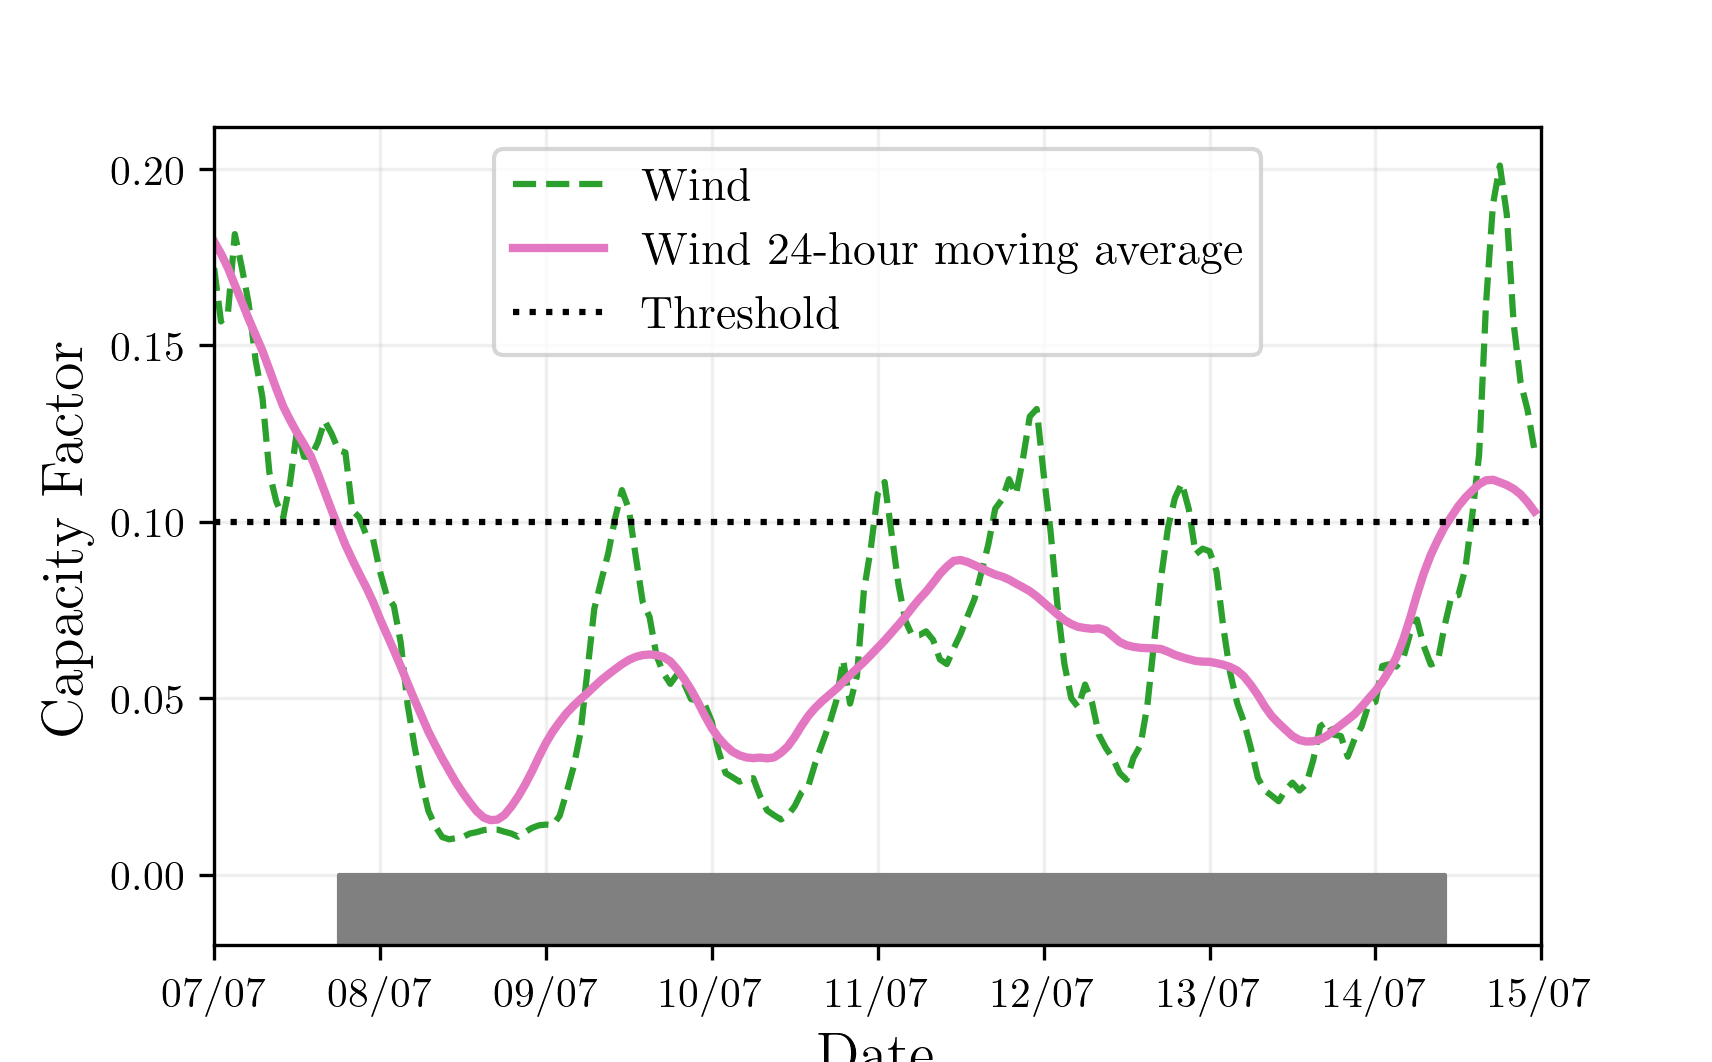
\includegraphics[width=\textwidth]{droughts_methodology}
	\caption{Wind time series of CF (red) and its 24-hour moving average (green) from the 7th to the 15th of July 2021. CF threshold (dashed black). The grey bar shows the period identified as a wind drought under our definition}
	\label{fig:find_res_droughts}
\end{figure}

Fig.~\ref{fig:find_res_droughts} illustrates the moving average identification method. When applying the moving average, this CF time series identifies a single event lasting 161 hours. In contrast, using the raw CF series would have resulted in three separate events, with durations of 36, 35, and 40 hours.

The moving average approach smooths out short-term fluctuations, so that brief periods above the threshold do not interrupt an otherwise continuous low-CF period. This means that a single hour above the threshold does not "break" a drought event if it is surrounded by prolonged low-generation hours. As a result, fewer but longer-lasting drought events are identified, which may better reflect real-world conditions where energy supply constraints persist over extended periods.

\section{Results}
\label{sec:Results}

\subsection{Verification}
\label{sec:verification}

Before going into the analysis of RES droughts, it is important to first verify the accuracy of the datasets used in this study. For the verification process, we use time-varying values of installed capacity to account for changes in RES development over the verification period. This step allows us to assess how well the datasets represent the production of renewable energy by comparing them against observed data.
	
\subsubsection{Wind Energy}
\label{sec:wind_verification}

The C3S-E datasets use the Vestas V136/3450 wind turbine power curve, (Fig.~\ref{fig:power_curve} a). The Atlite model allows the user to specify the power curve. We considered the 121 power curves available for download from Renewables.ninja~\cite{staffell2016wake}. For each power curve, Renewables.ninja also provide four associated smoothed power curves. The smoothing is done by using a Gaussian filter with different standard deviations that depend on the wind speed. A wind CF time series for Ireland for all wind turbine power curve options and all smoothings is generated. The performance of each wind turbine power curve is then, calculated based on four skill scores: correlation coefficient (CC), root mean square error (RMSE), mean bias error (MBE), and area under the curve. The area under the curve was calculated from histograms of the hourly CF values for the most recent decade, 2014-2023. Based on these metrics, the most representative power curve for Ireland was the Enercon E112.4500 power curve with the $0.3w$  smoothing filter.

\begin{figure}[!ht]
	\centering
	\includegraphics[width=\textwidth]{power_curve}
	\caption{a/ Power curves of the Enercon E112.4500 with a 0.3 smoothing filter used by Atlite (blue) and the Vestas V136/3450 used by C3S-E (orange) b/ Histograms of wind CF for Ireland from Atlite (blue), C3S-E (orange) and EirGrid (shaded)}
	\label{fig:power_curve}
\end{figure}

The smoothing of the wind turbine power curve represents losses due to the wake effect, which is important when modelling wind energy on larger scales. The histogram in Fig.~\ref{fig:power_curve}b shows that the C3S-E power curve tends to underestimate low CF values and overestimate higher ones, whereas the smoothed Atlite power curve more closely follows the recorded wind data from EirGrid.

\begin{figure}[!ht]
	\centering
	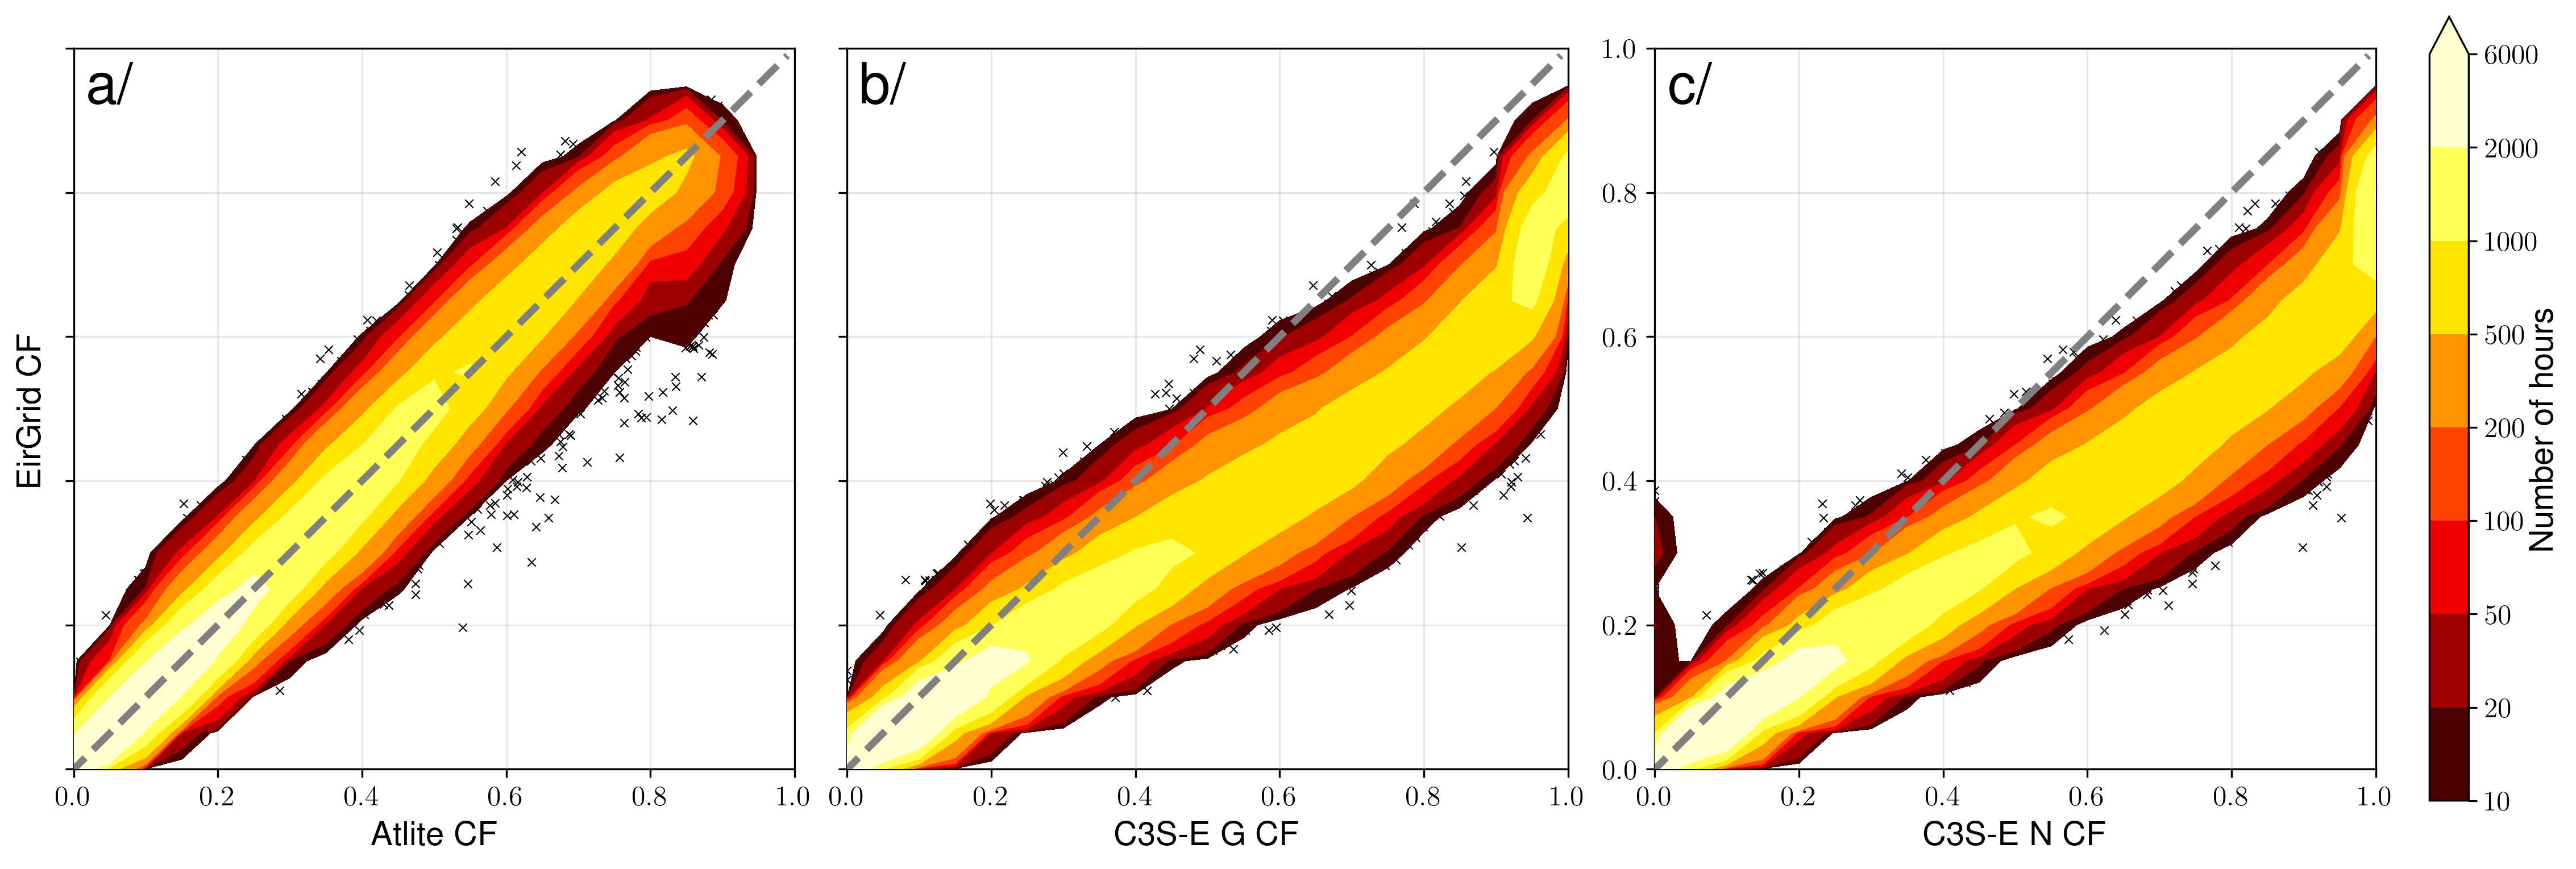
\includegraphics[width=\textwidth]{verification_wind_contour}
	\caption{Wind CF density plot of the observed EirGrid CF (vertical axes) and modelled (horizontal axes) CF data for the Atlite  (left panel), C3S-E G (central panel) and C3S-E N (right panel) models}
	\label{fig:wind_verification_contour}
\end{figure}

The effect of the differences in the power curves are also visible in Fig.~\ref{fig:wind_verification_contour} where the Atlite model shows good agreement with the EirGrid data. In contrast, the two C3S-E datasets tend to overestimate the EirGrid CF. This is confirmed by Table~\ref{tab:wind_skill_scores}, which shows that Atlite performs better than the C3S-E datasets for all three skill scores. 

\begin{table}[!ht]
	\centering
	\begin{tabular}{l|lll|}
		\cline{2-4}
		& \textbf{Atlite} & \textbf{C3S-E G} & \textbf{C3S-E N} \\ \hline
		\multicolumn{1}{|l|}{\textbf{CC}}   & 0.981           & 0.972            & 0.970            \\ \hline
		\multicolumn{1}{|l|}{\textbf{RMSE}} & 0.045           & 0.177            & 0.162            \\ \hline
		\multicolumn{1}{|l|}{\textbf{MBE}}   & -0.003          & 0.137            & 0.121            \\ \hline
	\end{tabular}
	\caption{Skill scores for wind for the three datasets compared to EirGrid data}
	\label{tab:wind_skill_scores}
\end{table}

Fig.~\ref{fig:bar_number_events_verification_wind} presents results for the average annual number of wind drought events during the 2014 to 2023 validation period. The figure shows that Atlite shows the best agreement overall with the observed frequency and duration of wind drought events. This pattern is particularly evident for shorter duration events, which are the most frequent.

\begin{figure}[!ht]
	\centering
	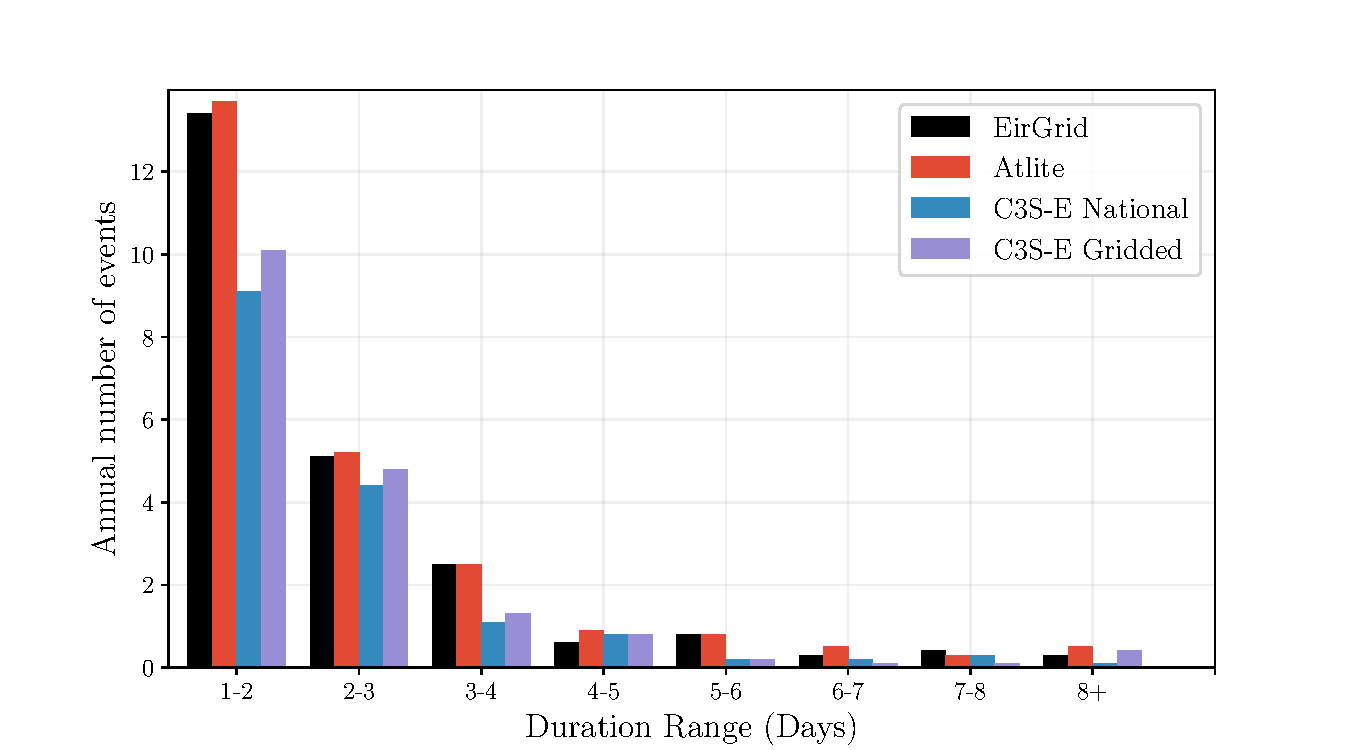
\includegraphics[width=\textwidth]{verification_wind_bar}
	\caption{Average annual number of wind drought events for EirGrid (black), Atlite (red), C3S-E G (blue), and C3S-E N (purple)}
	\label{fig:bar_number_events_verification_wind}
\end{figure}

\newpage
\subsubsection{PV Energy}
\label{sec:pv_verification}

The C3S-E datasets calculate PV generation multiple times using the same model with varying azimuth and tilt angles. The results are then aggregated based on a statistical distribution of module angles of Germany and then adapted to other European countries. Similarly to the wind CF verification, the Atlite model allows the user to select a given PV panel characteristics. In this study we have chosen to look at the three PV panels offered by in the Atlite model. Following the same methodology as in the previous section, we compare the three available models using four skill scores (CC, RMSE, MB, and area under the curve). Based on the best-performing metrics, we selected the Breyer PV panel model \cite{beyer2004pv}, using the Kaneka Hybrid panel option.

\begin{figure}[h!]
	\centering
	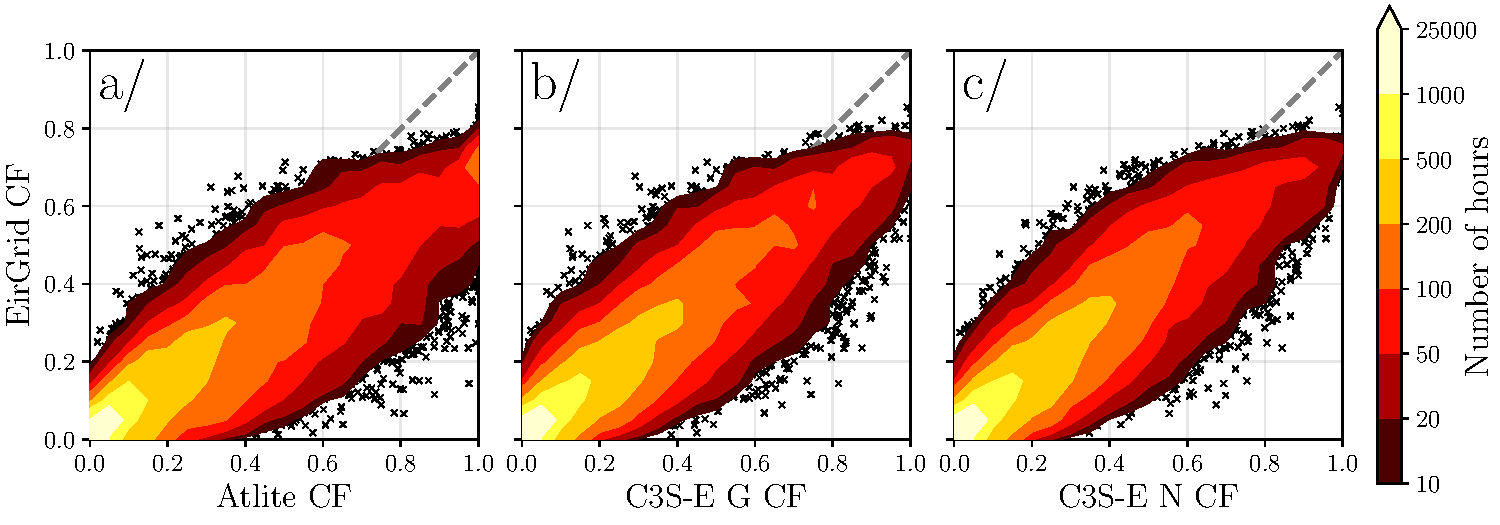
\includegraphics[width=\textwidth]{verification_pv_contour}
	\caption{PV 2D density plot of the observed EirGrid (vertical axes) and modelled (horizontal axes) CF series for the Atlite  (left panel), C3S-E G (central panel) and C3S-E N (right panel) models}	
	\label{fig:solar_verification_contour}
\end{figure}

Figure \ref{fig:solar_verification_contour} shows that the three datasets have a similar tendency of overestimating the CF compared to EirGrid. The skill scores presented in Table~\ref{tab:pv_skill_scores} indicate that C3S-E G performs best overall, with the lowest RMSE and a high correlation coefficient, suggesting a closer match to observed data. Atlite shows a slightly lower correlation and a higher RMSE, indicating larger deviations. All models show a slight positive bias, with Atlite exhibiting the most overestimation. These results reflect the broader challenges in accurately modeling PV, where variability is hard to capture. Nonetheless, C3S-E G’s lower RMSE suggests it may be more reliable for PV CF modeling in this context.

\begin{table}[!ht]
	\centering
	\begin{tabular}{l|lll|}
	\cline{2-4}
	& \textbf{Atlite} & \textbf{C3S-E G} & \textbf{C3S-E N} \\ \hline
	\multicolumn{1}{|l|}{\textbf{CC}}   & 0.921           & 0.931            & 0.931            \\ \hline
	\multicolumn{1}{|l|}{\textbf{RMSE}} & 0.119           & 0.090            & 0.113            \\ \hline
	\multicolumn{1}{|l|}{\textbf{MBE}}   & 0.046           & 0.027           & 0.021           \\ \hline
	\end{tabular}
	\caption{Skill scores for wind CF for the three datasets compared to EirGrid data}
	\label{tab:pv_skill_scores}
\end{table}

Fig.~\ref{fig:bar_number_events_verification_pv} shows the number of PV drought events in 2023 across different duration ranges. The figure reveals partial agreement between the three datasets and the EirGrid data, with consistent results observed for duration ranges of 1-2, 3-4, 7-8, and 8+ days. However, discrepancies appear in the other ranges, where the models diverge from the EirGrid data. The main challenge in validating PV data stems from the recent installation of a large share of Ireland’s PV capacity. Due to uncertainties in PV generation data during the first few months after each farm is connected, it is difficult to accurately determine the effective capacity. With over 60\% of the total PV capacity installed in 2023, these data uncertainties significantly impact the ability to perform rigorous validation for PV drought events. While the results are reasonably aligned in some ranges, the inherent challenges in PV data highlight the limitations of this verification.

\begin{figure}[!ht]
	\centering
	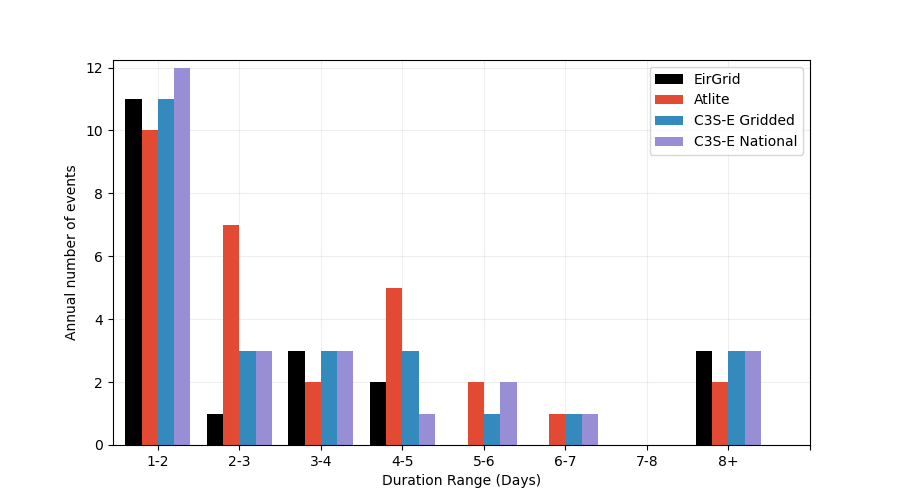
\includegraphics[width=\textwidth]{verification_pv_bar}
	\caption{Annual number of PV drought events for EirGrid (black), Atlite (red), C3S-E G (blue), and C3S-E N (purple) in 2023}
	\label{fig:bar_number_events_verification_pv}
\end{figure}

\newpage
\subsection{Analysis}
\label{sec:Analysis}

In this section, we evaluate RES drought events under two different scenarios with fixed installed capacities: the existing scenario, with 89\% of wind capacity (6.7 GW) and 11\% of PV capacity (0.6 GW), and a balanced scenario, where wind capacity comprises 53\% (9 GW) and PV capacity increases to 47\% (8 GW). Both scenarios are driven by 45 years of ERA5 data. Using the RES drought identification process described earlier (Section~\ref{sec:res_drought}), we first analyse wind and PV droughts separately before presenting the results for combined (wind + PV) RES droughts.

\subsubsection{Annual Number of RES Droughts}

The first part of the analysis examines the annual number of RES drought events across the three datasets. 

For wind (Fig.~\ref{fig:boxplot_number_events}a), the number of events decreases as the duration range increases, with very few events lasting more than seven days. For PV (Fig.~\ref{fig:boxplot_number_events}b), the number of events also declines as the duration range extends from one to eight days, followed by a slight increase for longer durations. This increase is due to extended low-generation periods occurring from November to March, depending on the dataset. When comparing wind and PV results (Fig.~\ref{fig:boxplot_number_events}a \& Fig.~\ref{fig:boxplot_number_events}b), the median, first, and third quartiles for PV are consistently higher or equal to those for wind, across all duration ranges and datasets. This is due to PV's typically lower CF compared to wind, especially in a region like Ireland where solar potential is limited. PV generation is also zero at night and constrained by the daily solar cycle, leading to a naturally higher frequency of RES droughts in PV compared to wind.

The bottom panels show the combination of wind and PV under the  two capacity scenarios. In the existing RES installation scenario (Fig.~\ref{fig:boxplot_number_events}c), the identified RES droughts closely match those for wind alone, which is expected due to the dominance of installed wind capacity. In contrast, the balanced scenario (Fig.~\ref{fig:boxplot_number_events}d) shows a clear reduction in the number of drought events across all datasets and durations, with a decrease of the total number of events of 56\% for Atlite, 52\% for C3S-E G, and 50\% for C3S-E N. This reduction is attributed to the anti-correlation between wind and PV production throughout the year, a phenomenon well-documented in the literature \cite{kaspar2019drought} and discussed in further detail in the later analysis.

The median, first, and third quartiles for the Atlite dataset are consistently greater than or equal to those of the other two datasets, regardless of the duration range or type of renewable energy considered. This difference arises from the wind turbine power curve model used in the C3S-E datasets, which tends to overestimate the wind CF (Fig.~\ref{fig:wind_verification_contour}). As a result, the overall number of RES droughts is underestimated in the C3S-E datasets compared to Atlite.

\begin{figure}[!ht]
	\centering
	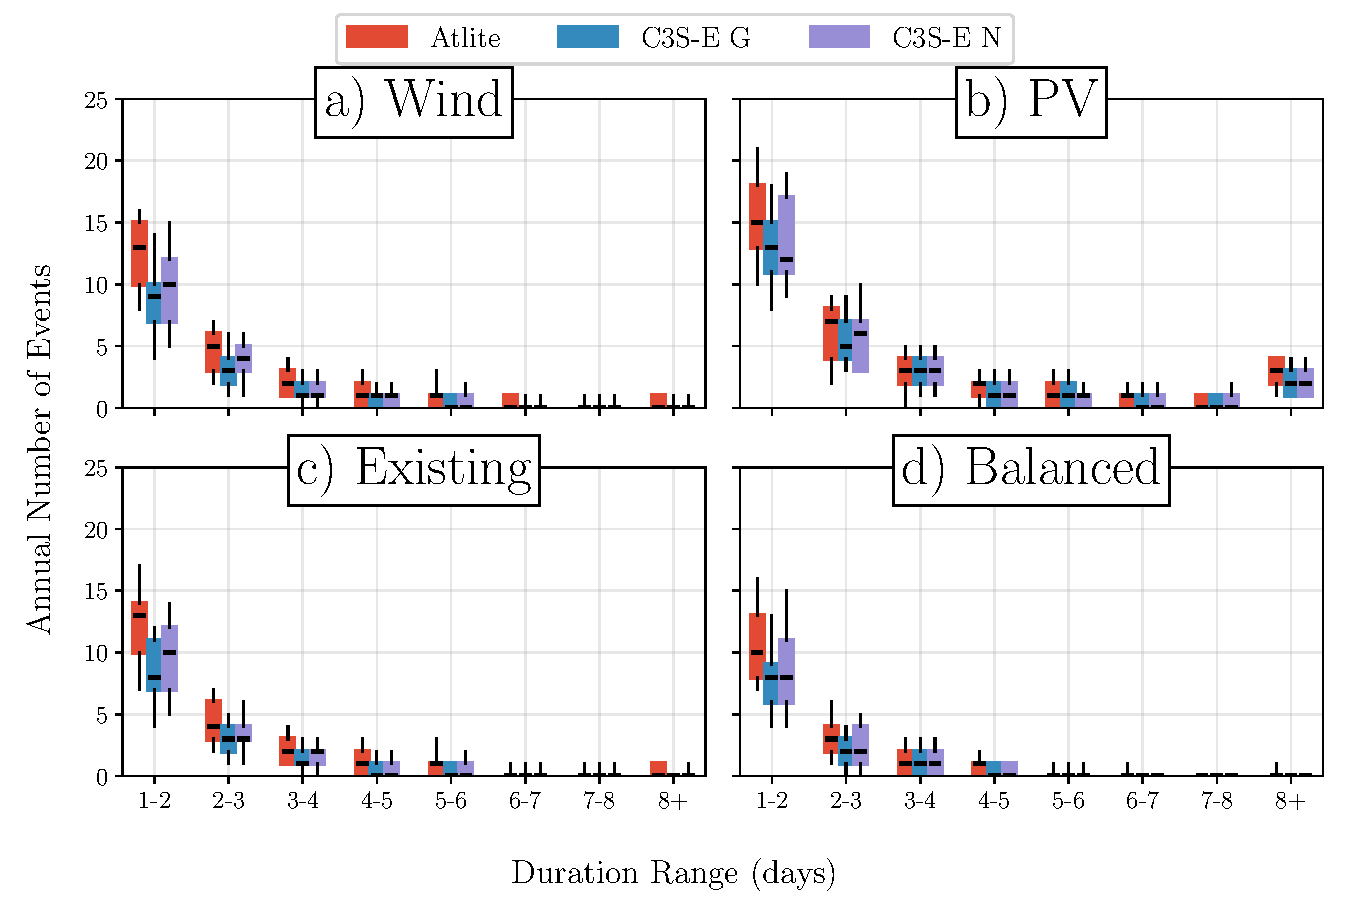
\includegraphics[width=\textwidth]{droughts_number_events}
	\caption{Annual number of RES droughts for a)~Wind, b)~PV, and the combination for the c)~current and d)~projected installed capacity for Atlite (red), C3S-E G (blue), and C3S-E N (purple). The x-axis represents duration ranges in days (lower bound included), while the y-axis indicates the annual number of events. The boxes display the first and third quartiles and the median is marked by a black line. The whiskers indicate the 5th and 95th percentiles}
	\label{fig:boxplot_number_events}	
\end{figure}

\newpage
\subsubsection{Return Periods of RES Drought Duration}

The RES drought events identified over the 45-year period were used to calculate the return periods for different RES drought durations. A return period refers to the estimated average interval between occurrences of events with a specified duration or intensity. Fig.~\ref{fig:return_periods} illustrates the return periods for varying RES drought durations, highlighting how often different drought lengths are likely to occur across the datasets. This analysis provides insight into the frequency and likelihood of prolonged low-generation periods, which is crucial for evaluating the potential impact of RES droughts on energy reliability.

For wind (Fig.~\ref{fig:return_periods}a), the duration of RES droughts increases in a log-linear fashion across the three datasets. The log-linear trend indicates a predictable relationship between drought duration and occurrence, with longer RES droughts becoming exponentially less likely as duration increases. 

For PV (Fig.~\ref{fig:return_periods}b), Atlite behaves significantly different than the two C3S-E datasets. The Atlite results follow the ones for wind with a log-linear increase, but reach higher values in general with the longest event lasting forty days. For C3S-E G and C3S-E N, the duration of RES droughts increases in a log-linear pattern for events lasting less than 16 days. Beyond this duration, there is a sharp rise in drought duration for events up to a one-year return period. This sudden increase reflects the impact of winter on PV generation in Ireland, as PV output often remains below the CF threshold for extended periods during winter months. The difference between Atlite and the C3S-E datasets likely arises from how each model handles PV output near the threshold. Atlite appears to hover slightly above the threshold more frequently during these conditions, leading to shorter, more fragmented drought events. In contrast, C3S-E G and C3S-E N tend to fall below the threshold in similar conditions, resulting in longer continuous drought periods, especially during winter. This sensitivity to the threshold highlights how slight model differences can have substantial effects on drought duration estimates, particularly for PV in low-generation conditions.

For the existing installed capacity scenario (Fig.\ref{fig:return_periods}c), the return periods mirror those of wind (Fig.\ref{fig:return_periods}a), reinforcing that wind is the primary driver of drought patterns in the current energy mix. In the balanced scenario (Fig.~\ref{fig:return_periods}d), the return periods for RES droughts increase across all durations. For example, the return period for a five-day drought event extends from roughly six months to four years in the Atlite dataset, and from about fifteen months to around five years in the two C3S-E datasets. The return periods for Atlite align more closely with those of C3S-E in the balanced scenario compared to the existing one. This convergence is due to the reduced proportion of wind capacity in the balanced scenario, which lessens the impact of wind-specific characteristics. Notably, there is a greater difference in how each model represents wind generation than PV, meaning the balanced scenario reduces these wind-related discrepancies, bringing the datasets closer together.
 
Across Fig.\ref{fig:return_periods}a, c, and, d, the return periods in the Atlite dataset are consistently higher than those in the two C3S-E datasets. For instance, in the current scenario (Fig.\ref{fig:return_periods}c), an event with a one-year return period lasts six days in the Atlite dataset, compared to only five days in the C3S-E datasets. This difference underscores the importance of model selection when quantifying RES droughts, as each model’s assumptions and parametrisations significantly influences drought duration estimates. Additionally, in all four panels, the similarity between results from the two C3S-E datasets suggests that assumptions in the Atlite model—such as wind turbine power curve selection and PV panel specifications—have a greater impact on RES drought duration estimates than the precise geographic distribution of RES farms when studying the return periods of RES droughts.

\begin{figure}[!ht]
	\centering
	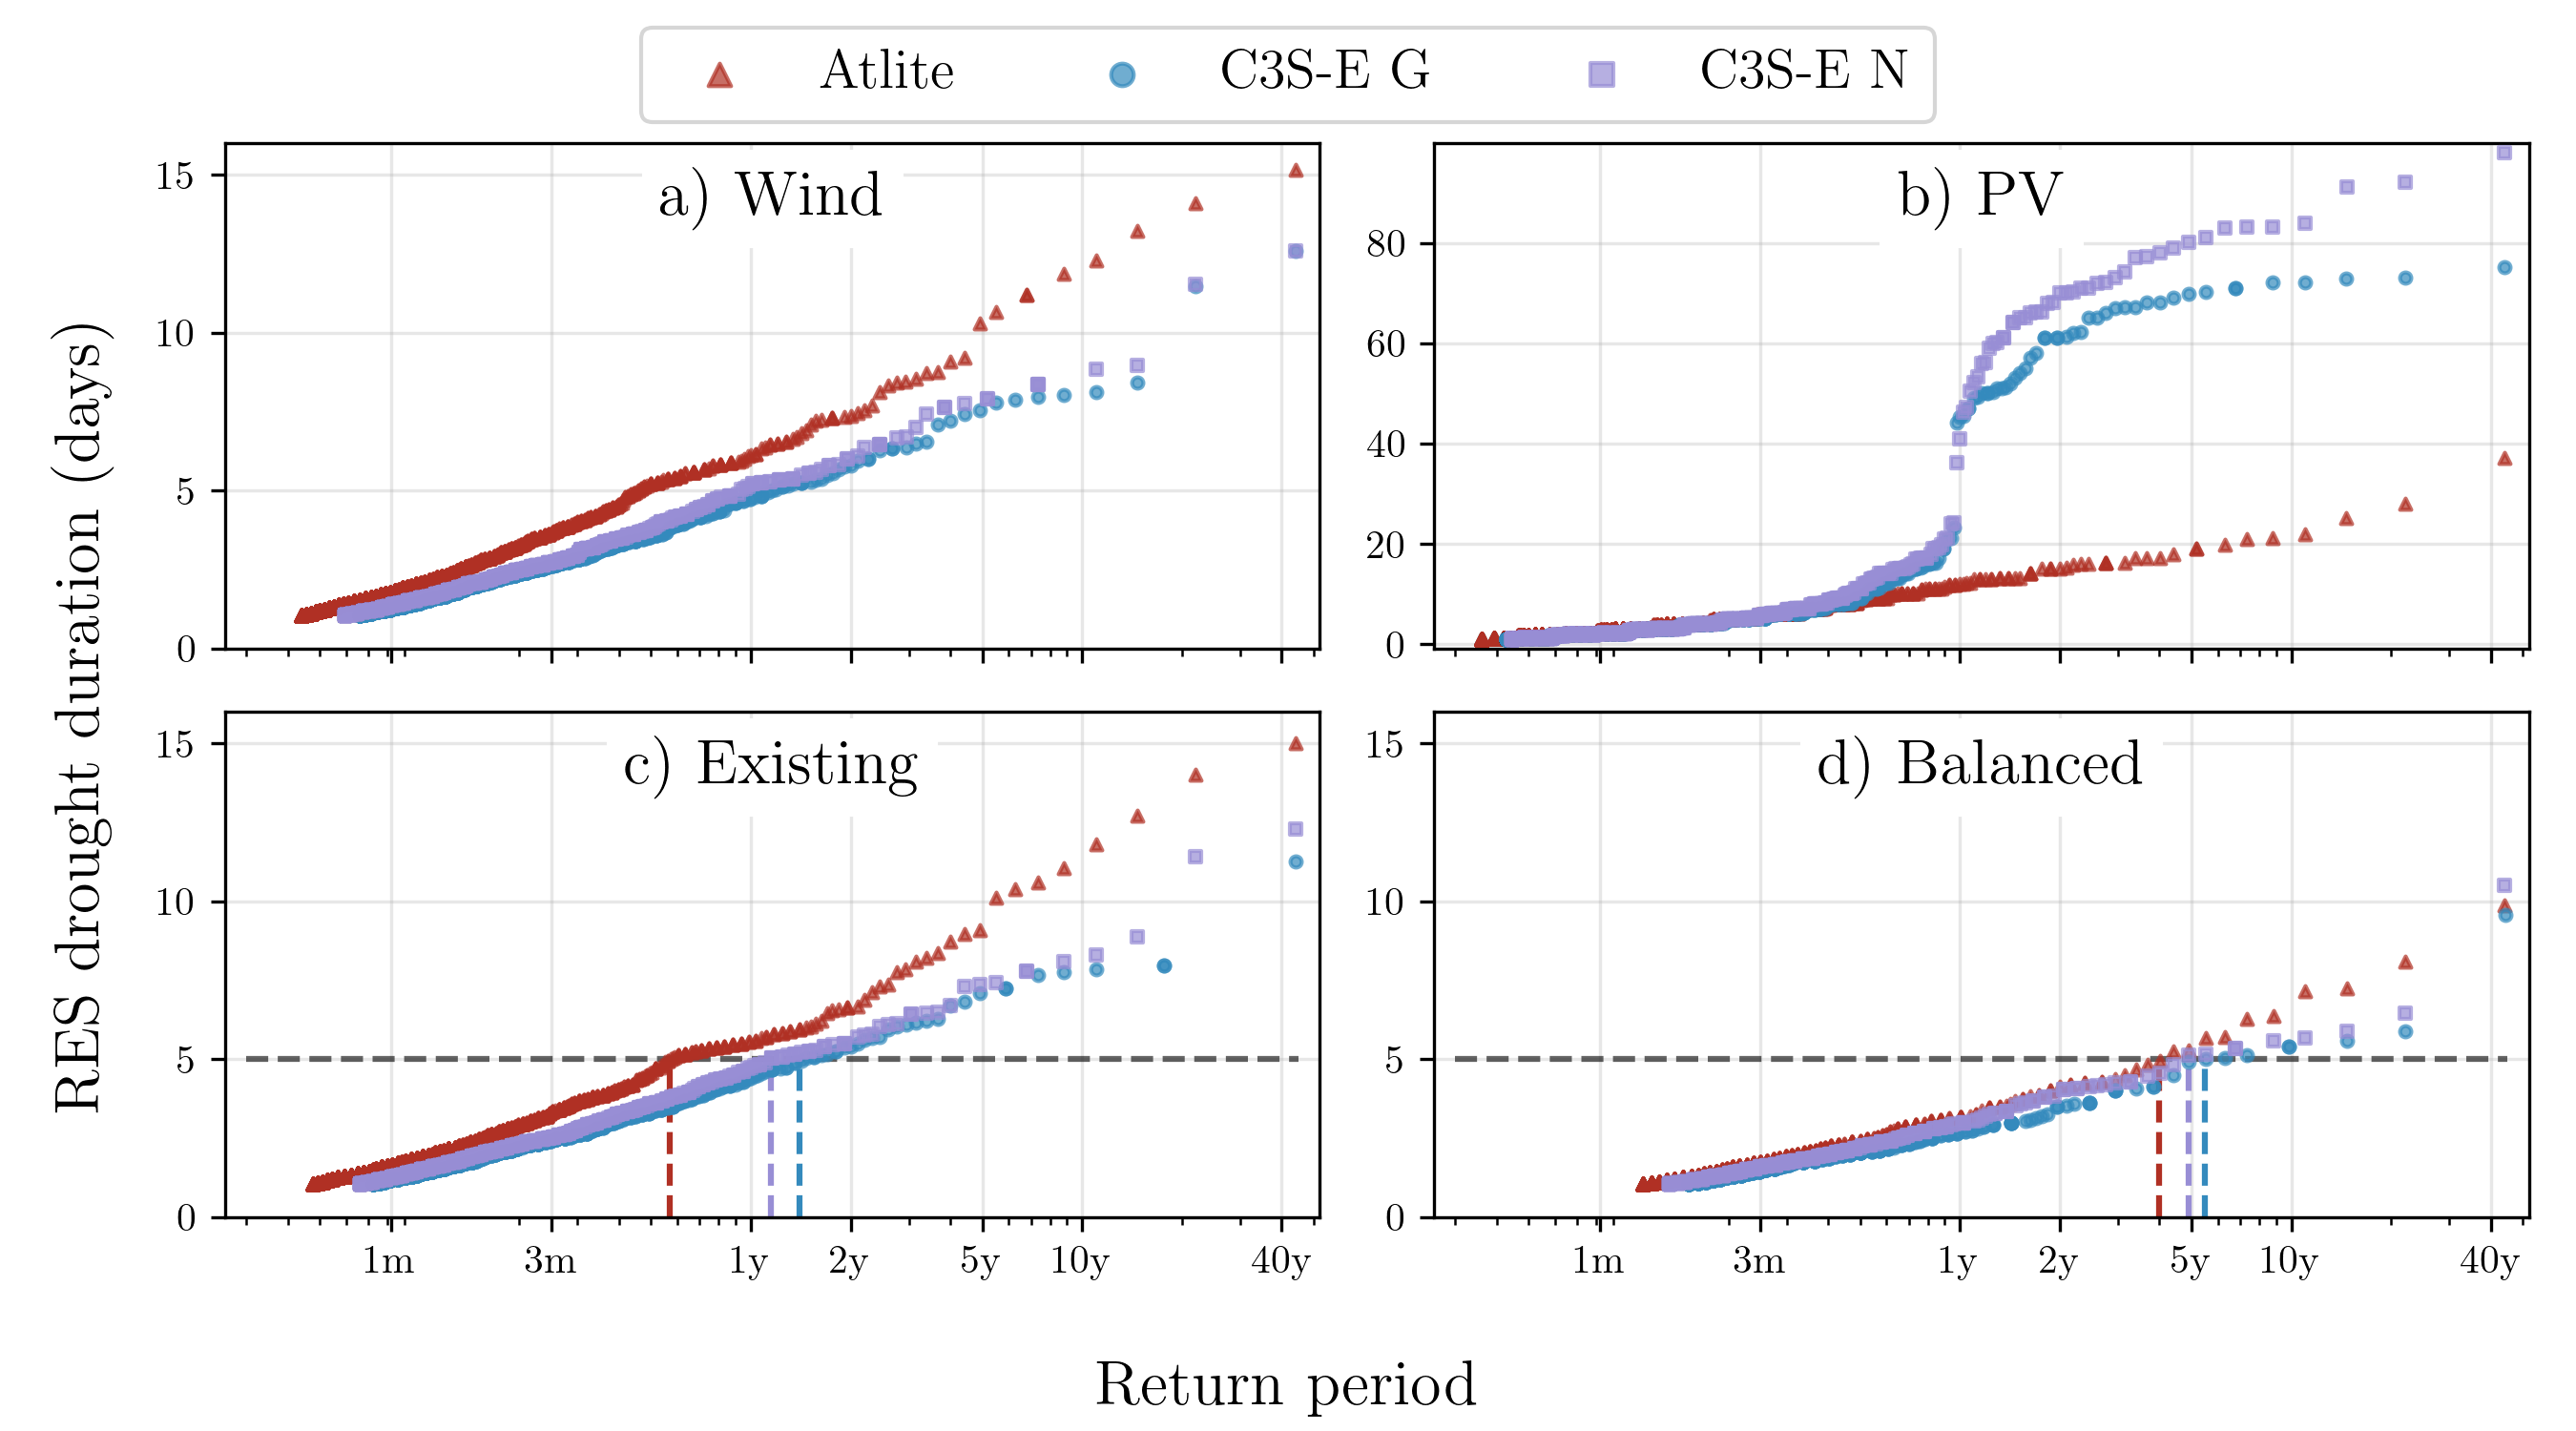
\includegraphics[width=0.9\textwidth]{droughts_return_periods}
	\caption{Return periods of the duration of RES droughts for a)~Wind, b)~PV, and the combination for the c)~current and d)~projected installed capacity, for Atlite (red), C3S-E G (blue), and C3S-E N (purple). The x-axis represents the return period time in a log-scale and the y-axis indicates the duration of RES drought associated with it. The horizontal dashed line in the two bottom panels marks the 5-day return period, with coloured vertical dashed marking its return period for each dataset.}
	\label{fig:return_periods}
\end{figure}

\newpage
\subsubsection{Seasonal Distribution of RES Droughts}

The seasonality of RES droughts is analysed by comparing the percentage of hours in each month classified as part of a RES drought. 

For wind (Fig.~\ref{fig:res_droughts_seasonality}a), RES drought percentages are higher in summer than in winter. In the Atlite dataset, for instance, an average of 24\% of hours in summer (JJA) are identified as RES droughts, compared to only 4\% in winter (DJF). This seasonal variation is influenced by the wind power curve model used to estimate CF, where the shape of the curve in lower wind speed regions (3-10 m/s) leads to significant differences in CF under low wind conditions. In contrast the results for PV (Fig.~\ref{fig:res_droughts_seasonality}b) show a higher percentage in winter, with RES droughts occurring over 60\% of the time regardless of the dataset. The Atlite results show a higher percentage of RES drought hours for wind, and a slightly lower percentage for PV, compared to the two C3S-E datasets. 

Similar to previous results, the existing installed capacity wind-PV combination (Fig.\ref{fig:res_droughts_seasonality}c) shows patterns comparable to the wind panel (Fig.\ref{fig:res_droughts_seasonality}a). However, in this panel, the number of hours classified as RES droughts in summer decreases slightly compared to the wind-only scenario. This reduction can be explained by the contribution of PV generation during the summer months in the existing scenario, even though it constitutes only 11\% of total capacity. Since the number of RES drought hours for PV in summer is near zero, this small contribution has a noticeable impact on reducing overall drought hours. In the projected scenario (Fig.~\ref{fig:res_droughts_seasonality}d), all three datasets show a reduction in monthly RES drought frequency. The balanced mix of wind and PV in this scenario reduces the seasonal signal, slightly increasing the percentage of RES drought hours in winter months while significantly decreasing it in summer. Annual reductions in median RES drought frequency are observed across the datasets, dropping from 14\% to 5\% for Atlite, from 8\% to 3\% for C3S-E G, and from 9\% to 4\% for C3S-E N.
 
\begin{figure}[!ht]
	\centering
	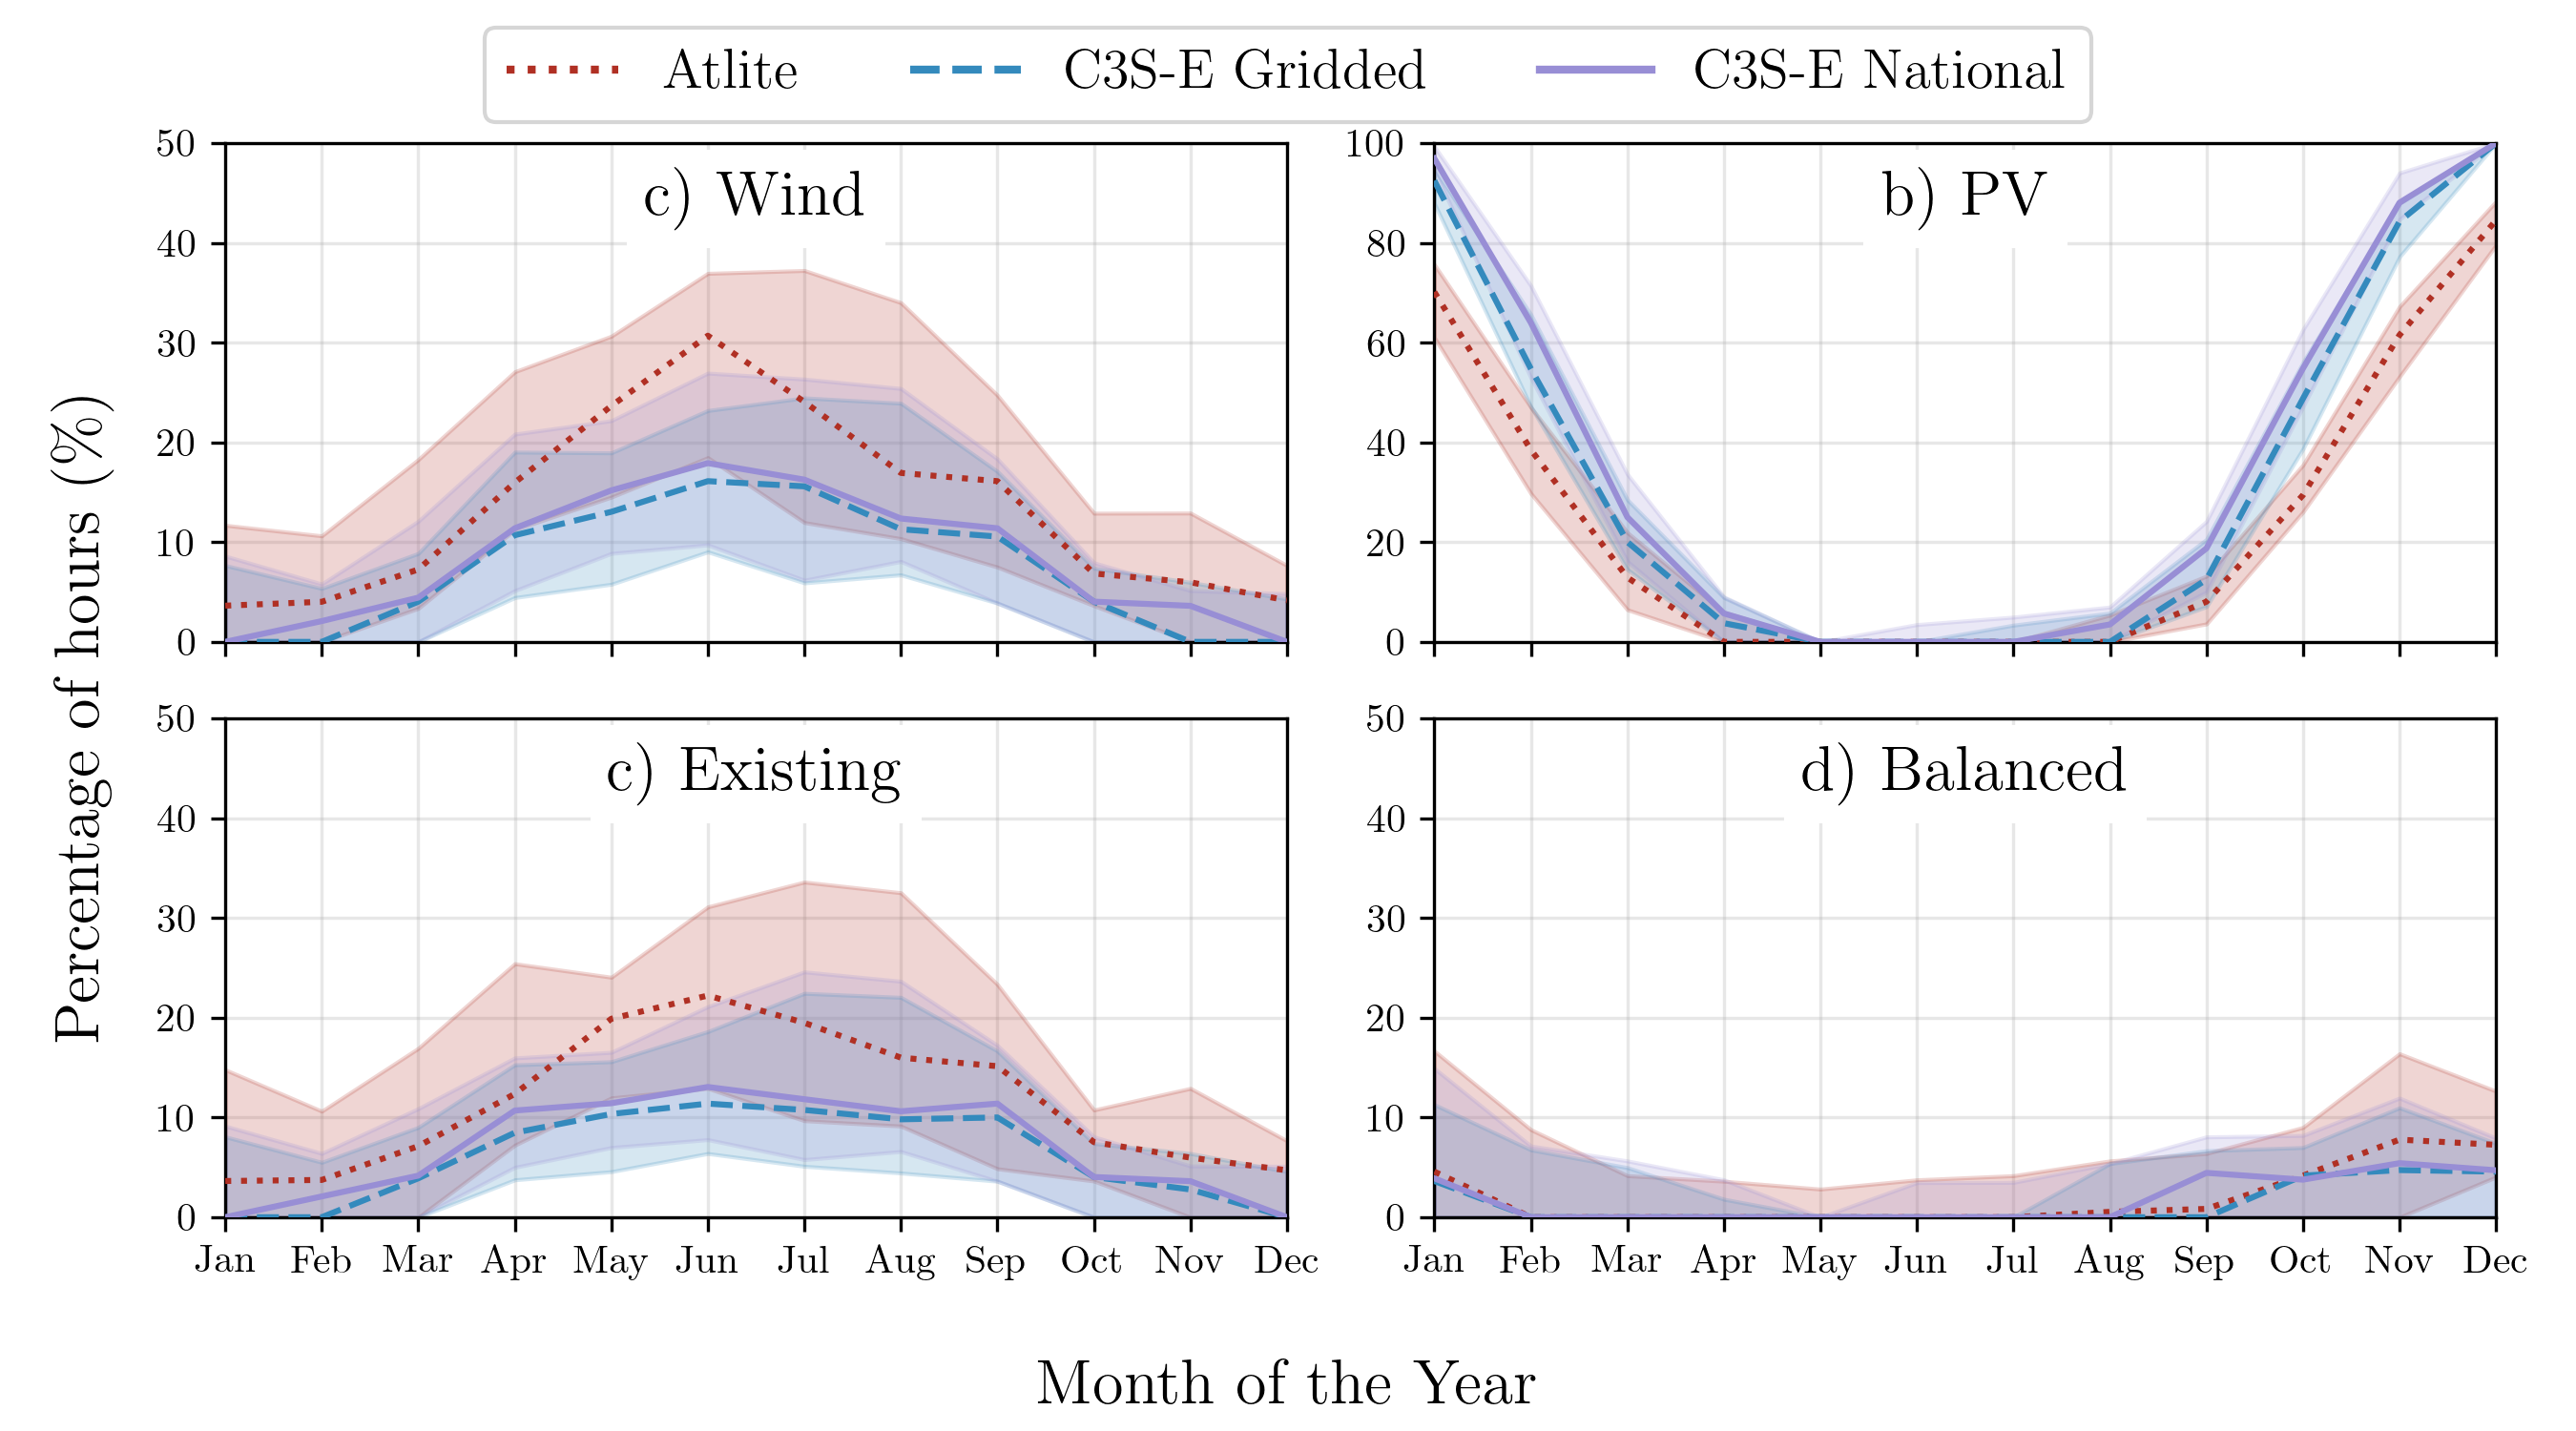
\includegraphics[width=\textwidth]{droughts_seasonality}
	\caption{Percentage of hours in a month identified as a RES drought for a)~Wind, b)~PV, and the combination for the c)~existing and d)~balanced installed capacity, for Atlite (red), C3S-E G (blue), and C3S-E N (purple). The x-axis represents the month of the year, and the y-axis indicates the percentage of hours. Lines correspond to the median values and the area between the first and third quartiles is shaded.}
	\label{fig:res_droughts_seasonality}
\end{figure}

\newpage
\subsubsection{Change of Threshold}

In this study, a threshold CF value of 0.1 has been used to identify RES droughts. To assess how sensitive the results are to this threshold, the annual number of events was calculated across a range of CF threshold values (Fig.~\ref{fig:number_days_threshold}).

Across all four panels, the results reveal a general trend: as the threshold increases, so does the number of identified events. This increase, however, is not uniform across datasets and energy sources, but the overall pattern remains consistent. When the threshold increases, smaller events merge into larger, less frequent events. Depending on the dataset, the number of events reaches a peak around or after a threshold of 0.2, and then gradually decreases until only a single event encompasses the entire time series.

Overall, the four panels indicate that regardless of the threshold applied, the Atlite dataset consistently identifies more events than the two C3S-E datasets, except for PV when the threshold is below 0.08. This finding suggests that Atlite, likely due to its more accurate representation of wind patterns in Ireland, captures more RES drought events that might be missed with different modeling assumptions in the C3S-E datasets.

\begin{figure}[!ht]
	\centering
	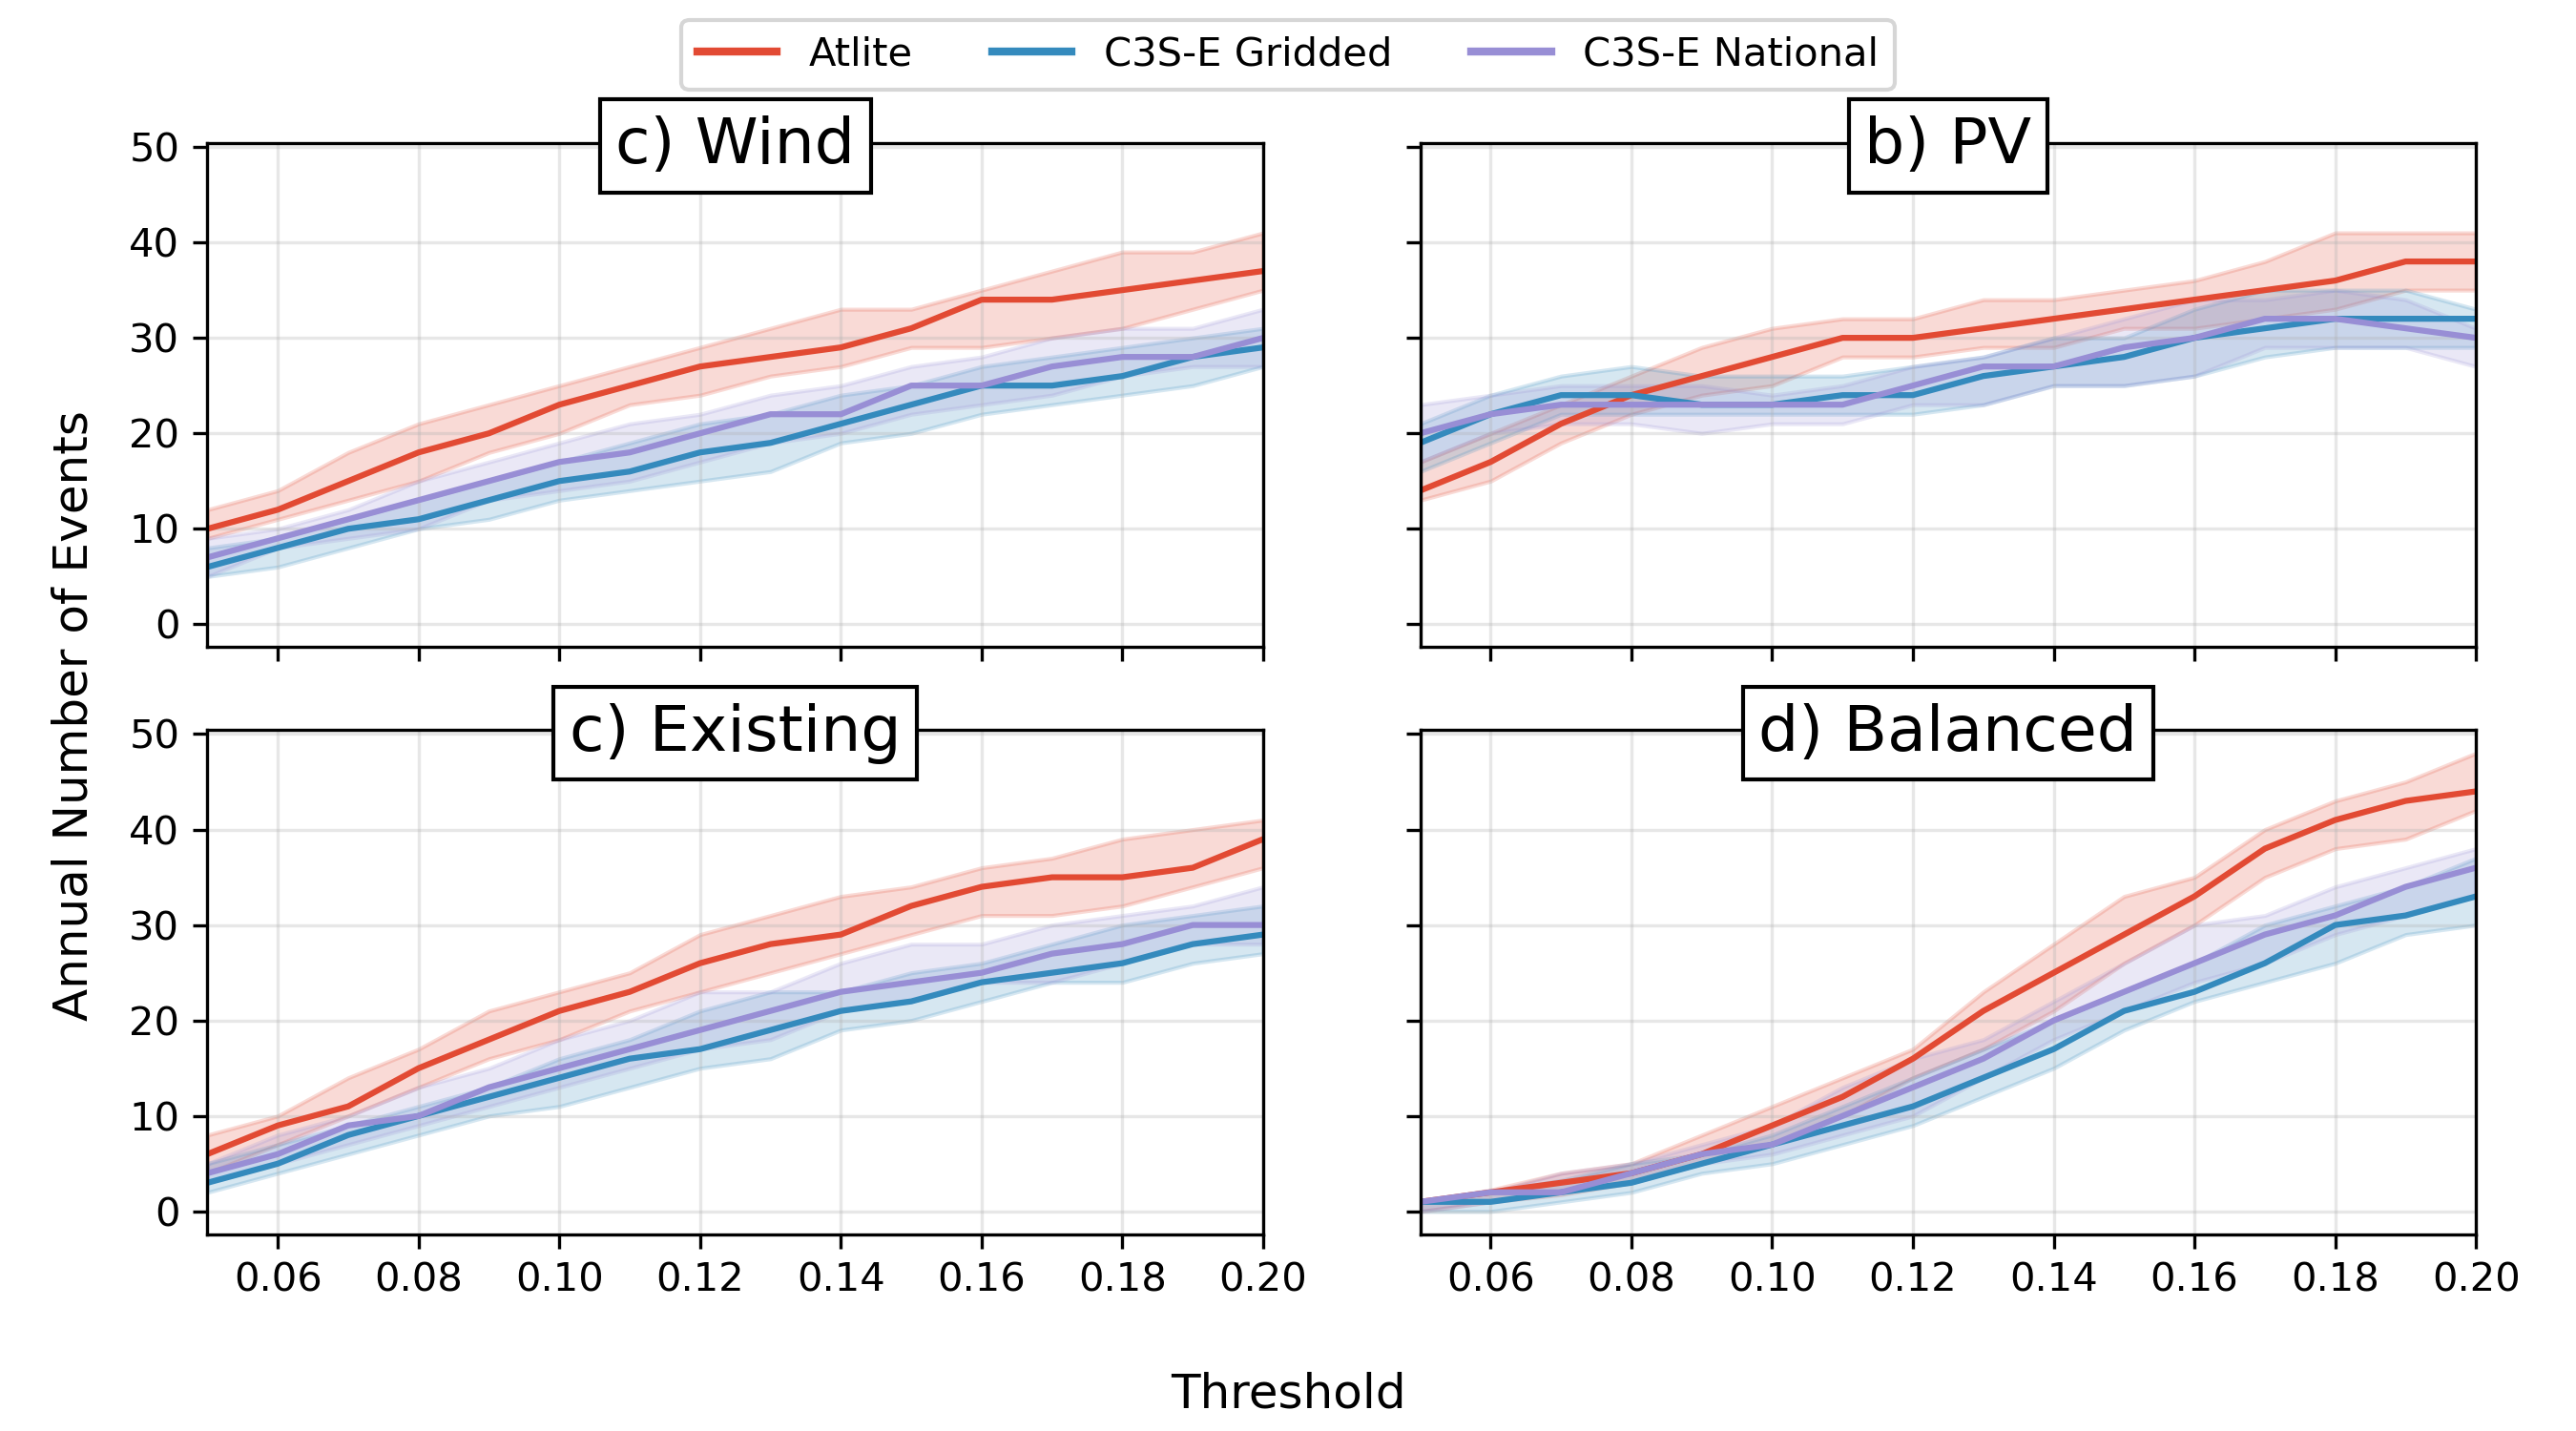
\includegraphics[width=\textwidth]{drouhgts_varying_threshold}
	\caption{Number of RES drought per year for a)~Wind, b)~PV, and the combination for the c)~current and d)~projected installed capacity, for Atlite (red), C3S-E G (blue), and C3S-E N (purple). The x-axis represent the threshold from 0.05 to 0.2 of the CF with a 0.01 increment. The y-axis indicates the annual number of events. Each line correspond to the median value and the first and third quartiles are shown in shaded area}
	\label{fig:number_days_threshold}
\end{figure}

\newpage
\section{Discussion and Conclusions}
\label{sec:Conclusion}

\begin{itemize}
	\item Remind differences between three datasets
	\begin{itemize}
		\item Atlite and C3S-E G: incorporate locations of RES farms
		\item Atlite models better follows EirGrid data (for Wind)
	\end{itemize}
	\item Point Arguments with examples from the figures
	\begin{itemize}
		\item The two C3S-E datasets show similar results
		\item Atlite stands out of these two datasets
	\end{itemize}
	\item Conclusion: Location of RES farms has less impact than the accuracy of modelling the CF!
	\\
	\item Impact of the 2030 scenario (Anti correlation between wind and PV) | Seasonality
	\\
	\item Risk for policymakers. The more accurate Atlite model produces more RES drought events and longer RES drought durations, an important consideration for risk-adverse decision making.
	\\
	\item Where to go next ?
	\begin{itemize}
		\item Looking at future climate data (Combine Climate and Energy scenarios)
		\item Studying broader region (Europe), which is more relevant as everything will be interconnected but more difficult as we will need to repeat verification for all EU countries
	\end{itemize}
\end{itemize}

This study has highlighted the key differences between the three datasets: Atlite, C3S-E G, and C3S-E N in their ability to model RES droughts. One of the most significant differences is how each dataset incorporates the specific locations of RES farms. Both Atlite and C3S-E G take into account the exact locations of wind and PV farms, which should, in theory, provide a more accurate representation of RES generation. However, our analysis shows that the Atlite dataset generally performs better, particularly in its wind generation estimates, where it closely follows the EirGrid data. This suggests that while the inclusion of RES farm locations is important, the accuracy of the CF modeling \textcolor{magenta}{I would say power curve model instead of CF modelling} used by Atlite may be the determining factor in its superior performance.\textcolor{magenta}{Superior how? Is finding more droughts superior or is it reproducing reality? I reckon it's the second, but make it explicit. Also, there is no explicit mention of PV, if you mention wind explicitly (which I agree on doing) I would add PV. Even though it is replacing that "However" with "Even though this is true for PV, our analysis shows that for wind..."}

When analysing the results, we found that the two C3S-E datasets (C3S-E G and C3S-E N) consistently show similar outcomes across various figures \textcolor{magenta}{I would not refer to them as figures, but as analysis or something like that. But if you do choose the word analysis, do not start the sentence with "When analysing the results..." and instead use something like "The results show..."} (Fig.~\ref{fig:boxplot_number_events},~\ref{fig:return_periods},~\ref{fig:res_droughts_seasonality}), suggesting that their differences in methodology have minimal impact on the results. In contrast, Atlite stands out in its ability to model wind generation, as evidenced by the more accurate correlation with EirGrid data seen in the verification process (Section \ref{sec:wind_verification}). This distinction is further underscored in the figures \textcolor{magenta}{Same as before, avoid referring to the figures. We do not discuss the result (that was done in results), we discuss what it implies}, where Atlite often reports higher or more accurate return periods and a greater number of RES droughts (Fig.~\ref{fig:boxplot_number_events},~\ref{fig:return_periods}), particularly in scenarios with increased PV capacity. \textcolor{magenta}{For me, the point of this paragraph is quite clear but does not really come across at the moment: Atlite is the best one at reproducing reality (as established in the previous paragraph). At the same time, a long-term analysis shows more droughts for Atlite than any other model. This means that model selection is key to correctly quantify the risk and avoid undersizing the reserve capacity.}

One of the most critical conclusions of this study is that the specific locations of RES farms, while important, have a lower impact on the accuracy of RES drought modelling than the precision of the CF models themselves. \textcolor{magenta}{Same as before, I would not refer to CF models, but instead wind power curve and PV panel models} Atlite's superior performance suggests that refining these models could lead to better forecasting and planning for RES droughts, which is crucial for energy security.

Looking to the balanced scenario, our analysis suggests a significant shift in the dynamics of RES droughts due to the anti-correlation between wind and PV generation. This scenario reveals the importance of seasonality in RES droughts (Fig.~\ref{fig:res_droughts_seasonality}), where a diversified energy portfolio that includes both wind and PV could decrease the frequency and duration of RES droughts.
\textcolor{magenta}{I would merge these two paragraphs into one. Here are my thoughts in order: 1. We have found how wind and PV together perform better than individually in terms of droughts. 2. A specific mention of seasonality and how it is reduced. 3. Mention how Ireland has a very wind-dependent system and how targets for PV are ambitious in the coming years, almost making wind and PV capacities equal (maybe not the phrasing but you see the point, putting forward the balance again). 4. Link to policymakers in terms of how meeting targets of installed capacity can help improve the energy security thanks to this diversification. 5. Close with the importance of the right model selection for RES drought assessment, especially as more renewable capacity comes into the system.}
For policymakers, the findings of this study highlight the risks of inadequate modelling and planning. Accurate RES drought forecasting is essential for ensuring energy security, especially as Ireland moves toward an ambitious renewable energy target.

In terms of future research, there are two main topics to explore. First, integrating future climate data with energy scenarios to better understand how climate change might affect RES droughts. Second, expanding the scope of the study to include Europe would provide a more comprehensive understanding of RES drought in an interconnected energy grid. However, this expansion would require extensive verification across all EU countries, making it a more complex but highly relevant challenge.

\newpage
\section{Acknowledgment}
Using the Climate Data Store. Thank EirGrid for the data and add a reference to the funding project or projects

\section{Funding information}

\section{Author contribution}

\bibliography{litrev}

\newpage
\section*{Appendix}


\end{document}
